\chapter{Realizacija sistema}\label{realizacija}
U ovom poglavlju nalazi se par odabranih realizacija stavki koje su predstavljale veći izazov za implementaciju, uz način na koji su izazovi prevaziđeni i navedene isečke izvornog koda.

\section{Uprošćavanje stabla parsiranja}
\label{sec:syntax}
Kao što je napomenuto, za parsiranje logičkih jednačina korišćen je parser bezkontekstne gramatike. U nastavku je izložena EBNF forma korišćene gramatike:
\begin{verbatim}
WellFormedFormula = QuantifiedFormula | Disjunction
QuantifiedFormula = SingleQuantifier QuantifiedFormula |
                    SingleQuantifier <'{'> QuantifiedFormula <'}'> |
                    SingleQuantifier <'{'> Disjunction <'}'>
<SingleQuantifier> = Quantifier | QuantifierNegation
Quantifier = FOREACH LITERAL | EXISTS LITERAL
QuantifierNegation = <'~'> Quantifier
Disjunction = Disjunction <'||'> Conjunction | Conjunction
Conjunction = Conjunction <'&&'> Implication | Implication
Implication = Implication <'=>'> Term | Term
Negation = <'~'> Term
Term = <'('> WellFormedFormula <')'> | Negation | Predicate | LITERAL
Predicate = PRED <'('> Arguments <')'>
<Arguments> = Arguments <','> Argument | Argument
Argument = LITERAL | Predicate

LITERAL = #'[a-z]+'
PRED = #'[A-Z][a-zA-Z]*'
FOREACH = <#'\\A'>
EXISTS = <#'\\E'>
\end{verbatim}
Prvi deo gramatike čine neterminali, a drugi deo čine terminali, definisani regularnim izrazima. Elementi u uglastim zagradama se \textbf{ne pojavljuju} unutar stabla parsiranja, ali inače čine deo gramatike.

Parser kao rezultat parsiranja izbacuje stablo parsiranja u \textit{Hiccup} formatu. Ovaj format sastoji se od ugnežđenih Clojure vektora. Svaki vektor obeležava čvor stabla. Prvi element svakog vektora jeste ključna reč koja obeležava terminal ili neterminal, a ostatak vektora su deca čvora, koja i sama mogu biti vektori. Radi pojašnjenja, daje se primer stabla parsiranja prostog logičkog izraza:
\begin{equation}
\label{eq:logic}
\forall x \; (\neg x \land y) \implies \mathit{Inv}(y, x)
\end{equation}
U datoj gramatici, ovaj izraz se zapisuje sa \verb|\A x {(~x && y) => Inv(y, x)}|, a stablo parsiranja ovog izraza je:
\begin{verbatim}
[:WellFormedFormula
 [:QuantifiedFormula
  [:Quantifier [:FOREACH] [:LITERAL "x"]]
  [:Disjunction
   [:Conjunction
    [:Implication
     [:Implication
      [:Term
       [:WellFormedFormula
        [:Disjunction
         [:Conjunction
          [:Conjunction
           [:Implication [:Term [:Negation [:Term [:LITERAL "x"]]]]]]
          [:Implication [:Term [:LITERAL "y"]]]]]]]]
     [:Term
      [:Predicate
       [:PRED "Inv"]
       [:Argument [:LITERAL "y"]]
       [:Argument [:LITERAL "x"]]]]]]]]]
\end{verbatim}
Kao što se može primetiti, dubina ugnežđivanja za prost logički izraz je veoma velika. Ovo je posledica činjenice da se u gramatici neki neterminali mogu zameniti nekim drugim, hijerarhijski nižim neterminalnom. Na primer, startni neterminal \texttt{WellFormedFormula} može da se zameni sa {\texttt{Disjunction}, a taj neterminal može da se zameni sa \texttt{Conjunction}, koji može da se zameni sa \texttt{Implication}, te onda sa \texttt{Term} itd.

Kako bi se olakšala dalja obrada stabla, i izbegla nepotrebna redundantnost, implementirana je funkcija koja skraćuje dubinu stabla, tako što eliminiše čvorove koji imaju samo jedno dete, sa određenim izuzecima. Skidaju se čvorovi koji predstavljaju neterminale osim \texttt{Negation} i \texttt{QuantifierNegation}, koji po definiciji imaju samo jedno dete. U listingu \ref{lst:simplify-tree} dat je izvorni kod ove funkcije.
\lstinputlisting[float, floatplacement=h, caption=Funkcija za uprošćavanje stabla parsiranja, label=lst:simplify-tree, language=Clojure]{listings/simplify-tree.clj}

Funkcija se oslanja na funkciju \texttt{transform} Instaparse biblioteke, koja prima mapu ključnih reči na funkcije. Ta funkcija potom prolazi kroz stablo, i menja čvorove sa rezultatima odgovarajućih funkcija. U ovom slučaju, za svaki neterminal mapira se povratna vrednost funkcije \texttt{simplify-tree*}, sa tim neterminalom kao argumentom. \texttt{simplify-tree*} pravi funkciju koja vraća prvo dete čvora, ukoliko čvor ima samo jedno dete, ili vraća originalni čvor, ukoliko čvor ima više dece.

Bitno je napomenuti da, u skladu sa duhom funkcionalnog programiranja, ne postoje stanja drveta parsiranja, već svaka operacija (poziv funkcije) rezultuje novim stablom. Uprošćeno stablo parsiranja koje vraća funkcija \texttt{simplify-tree} za izraz \ref{eq:logic} izgleda ovako:
\begin{verbatim}
[:QuantifiedFormula
 [:Quantifier [:FOREACH] [:LITERAL "x"]]
 [:Implication
  [:Conjunction [:Negation [:LITERAL "x"]] [:LITERAL "y"]]
  [:Predicate [:PRED "Inv"] [:LITERAL "y"] [:LITERAL "x"]]]]
\end{verbatim}

Dobijeno stablo je daleko prostije od početnog, i pogodno za dalju transformaciju. Zbog ovoga je prvi korak pri svođenju na KNF uprošćavanje stabla, što se može videti u telu funkcije \texttt{wff->cnf} (\ref{lst:wff}). Ova funkcija svodi datu jednačinu na KNF formu i koristi \textit{threading} Clojure makro da bi ,,provukla'' stablo kroz transformišuće funkcije.
\lstinputlisting[float, floatplacement=h, caption=Funkcija za svođenje na KNF formu, label=lst:wff, language=Clojure]{listings/wff.clj}

\section{Prilagođivanje HTML stranica za neke statusne kodove}
Doslednom izgledu veb aplikacije umnogome doprinose prilagođene stranice u slučaju da resurs nije nađen (status 404) ili da se dogodila neka interna greška (status 500). U slučaju greške, takođe je korisno prikazati i potpis steka korisniku kako bi administratori imali više informacija za otklanjanje problema.

\lstinputlisting[float, floatplacement=h, caption=Implementacija prilagođene 404 stranice, label=lst:routes, language=Clojure]{listings/routes.clj}
Jetty nudi podrazumevane stranice koje se vraćaju u ovakvim slučajevima, koje nisu u skladu sa izgledom izrađene veb aplikacije. Međutim, željeno ponašanje je moguće definisati preko Compojure ruta. Compojure rute se razrešavaju redom kojim su navedene. Ukoliko se nijedna ruta ne poklopi sa zahtevom, Compojure se obraća Jetty serveru, koji onda vraća 404 status sa podrazumevanom stranicom. Umetanjem posebne rute \texttt{compojure.route/not-found}, koja prihvata sve zahteve, na kraj liste ruta, obezbeđeno je izvršavanje hendlera za te rute ukoliko se nijedna ruta pre nje ne poklopi sa zahtevom. Ova ruta implementira prost hendler koji vraća prilagođenu 404 stranicu. Kod je dat na listingu \ref{lst:routes}.

\lstinputlisting[float, floatplacement=h, caption=Implementacija prilagođene 500 stranice, label=lst:exc, language=Clojure]{listings/exc.clj}
Situacija za stranicu sa greškom je malo komplikovanija, jer se ona pojavljuje ukoliko je došlo do neočekivane greške, na primer, neuhvaćenog izuzetka. Takođe, trik sa rutama ovde ne pomaže, jer se izuzeci koji su prošli van hendlera hvataju unutar Jetty koda. Ovde u pomoć uskače Compojure koncept koji se naziva \textit{middleware}. Prosto rečeno, middleware je funkcija omotač koja prva dobija kontrolu toka, poziva obmotani hendler, a potom dobija nazad kontrolu toka kada se hendler izvrši. Ovakva funkcija ima mogućnost da promeni strukturu zahteva pre nego što se on prosledi hendleru, ili da promeni ono što je hendler vratio kao odgovor.

Vredno je napomenuti da se Compojure middleware funkcije mogu obmotavati jedna oko druge. Ovaj koncept jako podseća na dekoratore u OOP svetu.

Za potrebe prikazivanja prilagođene stranice u slučaju greške, napravljena je middleware funkcija \texttt{wrap-catch-exceptions} koja obmotava sve rute, a koja hvata sve tipove izuzetaka koji se dese u unutrašnjim hendlerima. Ukoliko se uhvati takav izuzetak, kao odgovor se vraća status 500, a kao telo se navodi string koji sadrži informacije o izuzetku, zajedno sa potpisom steka.

Pored ove funkcije postoji i \texttt{wrap-500} middleware, koji presreće sve odgovore sa statusnim kodom 500, telo menja punom HTML prilagođenom stranicom, i postavlja neophodna HTML zaglavlja. Izvorni kod je priložen u listingu \ref{lst:exc}, a izgled obe stranice se može videti na slici \ref{fig:exc}.

Autor je prvobitno napravio previd time što je hvatao samo izuzetke tipa \texttt{java.lang.Exception}, pa se ponekad desilo da ,,isplivaju'' izuzeci koji nasleđuju klasu \texttt{Throwable}. Tada bi se prikazala standardna Jetty stranica za greške.
\begin{figure}[hb]
\centering
\fbox{
\includegraphics[width=0.95\textwidth]{404}}
\fbox{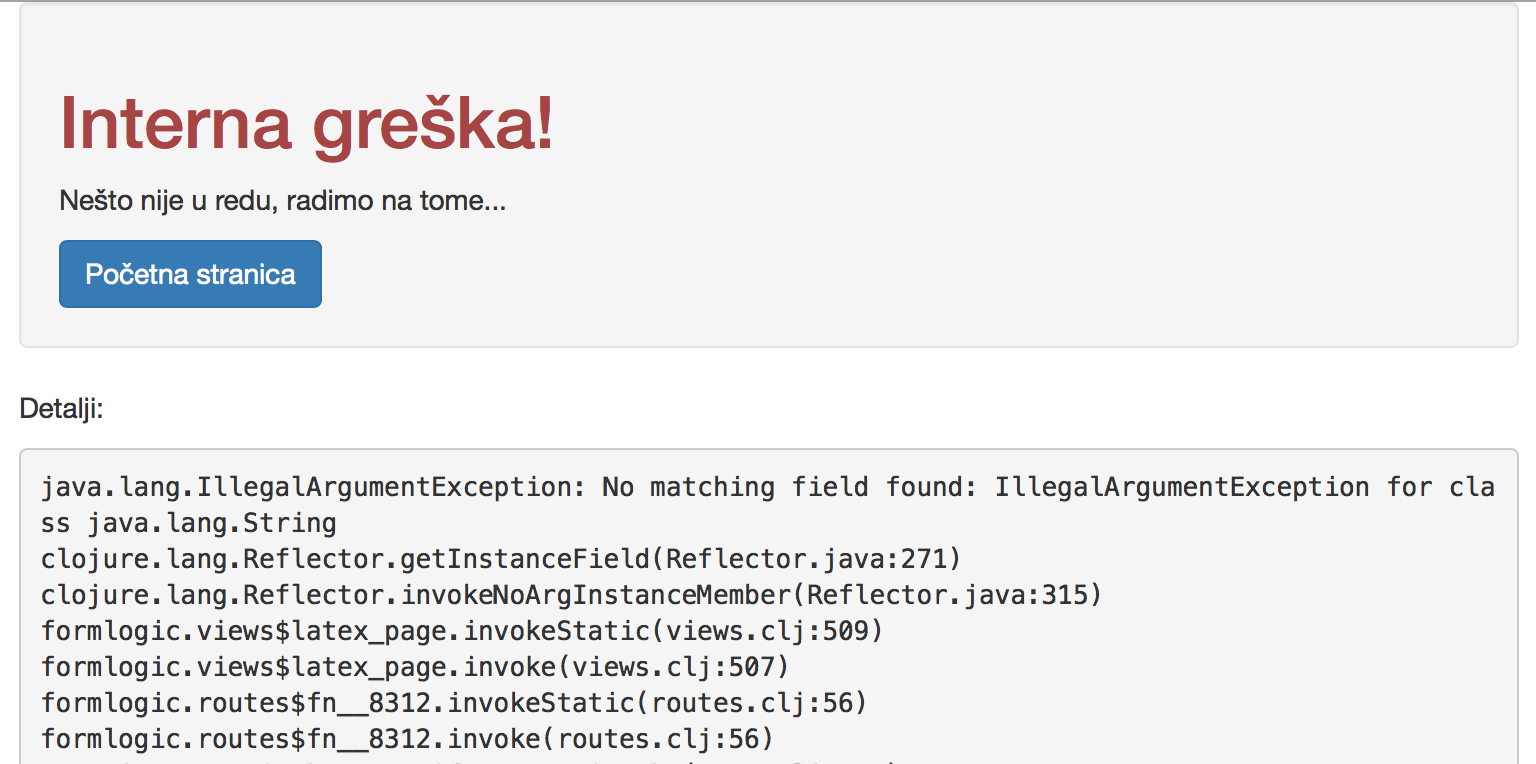
\includegraphics[width=0.95\textwidth]{500}}
\caption{Izgled prilagođenih stranica za statusne kodove 404 (\textit{gore}) i 500 (\textit{dole})}
\label{fig:exc}
\end{figure}

\section{SQL upit za dohvatanje završenih testova}
Na početnoj administratorskoj stranici moguće je dohvatiti sve završene testove na osnovu email naloga studenta ili imena testa. Za svaki test treba sračunati i procenat uspešnosti.

Ova operacija uključuje nekoliko akcija:
\begin{itemize}
\item dohvatiti završene test na osnovu primarnog ključa studenta ili testa iz tabele \texttt{assignment\_progress},
\item dohvatiti ukupan broj pitanja za svaki pronađeni test - ovo su statički podaci koji se nalaze u shemi \texttt{static},
\item dohvatiti ukupan broj pitanja na koja je student dao tačan odgovor iz tabele \texttt{question\_progress}, i, konačno,
\item izdvojiti i sračunati relevantne podatke i poslati ih nazad klijentu
\end{itemize}

\lstinputlisting[float, floatplacement=h, caption=SQL upit za dovlačenje završenih testova, label=lst:query, language=SQL]{listings/get.sql}
Umesto pozivanja pojedinačnih upita za svaki od ovih koraka, autor se odlučio za pristup gde će svi podaci biti dohvaćeni odjednom, u svom finalnom obliku. Za ovaj podvig je korišćena funkcionalnost Postgres-a pod imenom \textit{Common Table Expressions} (CTE). Ona omogućava pravljenje pod-upita unutar jednog upita, koje je moguće referencirati iz glavnog upita, i koristiti kao punopravne tabele. CTE izraze je takođe moguće referencirati i iz drugih CTE izraza. Osim ovoga, podržavaju i rekurziju.

Implementirani upit dat je u listingu \ref{lst:query}. Postoje tri CTE izraza koji dohvataju određene komponente neohodne za konstrukciju konačnih rezultata:
\begin{enumerate}
\item Prvi CTE dovlači gotove progrese (instance testa) za određeni test. Kriterijum završenog testa jeste da je kolona \texttt{completed\_at} popunjena.
\item Drugi CTE za svaki red iz prvog dovlači progres za sva pitanja za tu instancu testa iz \texttt{question\_progress} tabele. Ovaj upit ih nakon toga grupiše preko \texttt{GROUP BY} klauzule u dva reda po progresu, po jedan za svako stanje \texttt{boolean} kolone \texttt{correct}, i broji sve redove koji su na ovaj način grupisani. Rezultat se nalazi u \texttt{cnt} koloni. Na ovaj način su za svaku instancu testa prebrojani tačni i netačni odgovori. Drugi CTE ima ukupno $2 \times N$ redova, gde je $N$ broj redova u prvom CTE izrazu.
\item Treći CTE prosto sabira \texttt{cnt} kolonu za svaki progres iz drugog CTE izraza i rezultat stavlja u \texttt{total} kolonu. Ovo postiže tako što redove grupiše po ID koloni. Treći CTE ima $N$ redova, po jedan za svaki red iz prvog CTE izraza.
\end{enumerate}

Konačno, rezultat se dobija tako što se iz prvog CTE izraza pokupe ID progresa, datum početka izrade, datum kraja izrade i email nalog studenta (ovo se zapravo dobija preko \texttt{INNER JOIN}-a sa \texttt{user} tabelom na koloni \texttt{user\_id}). Poslednja kolona sadrži ocenu uspešnosti koja se sračunava kao količnik odgovarajuće kolone \texttt{cnt} iz drugog CTE izraza, za koju je \texttt{correct} tačan, i ukupnog broja pitanja iz trećeg CTE izraza, tj. odgovarajuće kolone \texttt{total}. Na kraju se rezultati sortiraju prema datumu predaje testa, i vraćaju klijentu u JSON formi.

Prva verzija upita je odgovarajući red iz drugog CTE izraza birala preko izraza \texttt{WHERE questions.correct = true} u glavnom upitu, a drugi CTE se stapao sa prvim preko \texttt{INNER JOIN}-a. Međutim, na ovaj način su preskakani testovi na kojima studenti nisu odgovorili tačno ni na jedno pitanje. Rešenje je bilo da se koristi \texttt{LEFT OUTER JOIN} sa drugim CTE izrazom, uz dodatno ograničenje da se tabele stapaju samo za redove gde je \texttt{correct} kolona označena kao tačna. Ova vrsta stapanja će za testove gde nema nijedno tačno pitanje umetnuti \texttt{NULL} vrednosti na mesta gde fale kolone, a \texttt{COALESCE} unutar izraza za računanje uspešnosti će se pobrinuti da se takva vrednost pretvori u nulu u aritmetičkom izrazu.

\section{Raspakivanje Postgres nizova}
Atributi nekih entiteta u bazi su pohranjeni kao nizovi, na primer, kolone \texttt{choices} i \texttt{answers} unutar \texttt{static.question} tabele. Funkcije koje učitavaju takve entitete iz baze, generisane od strane YeSQL biblioteke na osnovu SQL skripti, vraćaju rezultate u vidu Clojure mapa. Međutim, nizovi unutar tih mapa se vraćaju kao instance \texttt{org.postgresql.jdbc4.Jdbc4Array} klase. Kao primer je naveden izlaz funkcije \texttt{db/find-questions-by-task-id}:
\begin{verbatim}
({:answers #<org.postgresql.jdbc4.Jdbc4Array@3a1205f7 {2}>,
  :body "Koje je boje nebo?",
  :choices #<org.postgresql.jdbc4.Jdbc4Array@29ca0b4d
  {zute,crvene,plave}>,
  :id 1,
  :ord 1,
  :task_id 1,
  :type "single"}
 {:answers #<org.postgresql.jdbc4.Jdbc4Array@242f86ce {0,1,4}>,
  :body "Šta od navedenog NIJE satelit?",
  :choices #<org.postgresql.jdbc4.Jdbc4Array@6e8b2491
  {Jupiter,Demetra,Io,Kalisto,Orfej}>,
  :id 2,
  :ord 2,
  :task_id 1,
  :type "multiple"}
 {:answers #<org.postgresql.jdbc4.Jdbc4Array@441ca90a {0}>,
  :body "Kako se zove glavni grad Estonije?",
  :choices #<org.postgresql.jdbc4.Jdbc4Array@3df542a7 {Talin}>,
  :id 3,
  :ord 3,
  :task_id 1,
  :type "fill"})
\end{verbatim}
Problem nastaje ukoliko se nad vrednostima polja koja predstavljaju pomenute instance pokuša pozvati metoda \texttt{getArray()}. Po JDBC dokumentaciji\footnote{\url{https://docs.oracle.com/javase/tutorial/jdbc/basics/array.html}}, tada dolazi do materijalizacije elemenata niza, tj. tada se oni zapravo dovlače iz baze. Međutim, ukoliko se ova metoda pozove van JDBC transakcije, baca se izuzetak.

\lstinputlisting[float, floatplacement=h, caption=Funkcija za raspakivanje vrednosti JDBC nizova unutar transakcije, label=lst:array, language=Clojure]{listings/array.clj}
Rešenje ovog problema jeste da se vrednosti unutar JDBC niza raspakuju dok još traje transakcija. YeSQL ima mogućnost da se funkcijama koje predstavljaju upite prosledi funkcija za transformisanje redova. Ova funkcija se izvršava nad svakim dovučenim redom pre nego što se transakcija zatvori, i vraća rezultat obrade. Stoga je implementirana funkcija \texttt{db/unwrap-arrays}, priložena u listingu \ref{lst:array}, koja prolazi kroz sve unose mape koja predstavlja jedan red iz tabele i raspakuje JDBC nizove, ukoliko naiđe na njih.

Kada se pomenuta \texttt{db/find-questions-by-task-id} funkcija pozove sa funkcijom za transformisanje redova \texttt{db/unwrap-arrays}, na mestu JDBC nizova dobijaju se standardni Clojure vektori, unutar kojih su raspakovane vrednosti:
\begin{verbatim}
({:answers [2],
  :body "Koje je boje nebo?",
  :choices ["zute" "crvene" "plave"],
  :id 1,
  :ord 1,
  :task_id 1,
  :type "single"}
 {:answers [0 1 4],
  :body "Šta od navedenog NIJE satelit?",
  :choices ["Jupiter" "Demetra" "Io" "Kalisto" "Orfej"],
  :id 2,
  :ord 2,
  :task_id 1,
  :type "multiple"}
 {:answers [0],
  :body "Kako se zove glavni grad Estonije?",
  :choices ["Talin"],
  :id 3,
  :ord 3,
  :task_id 1,
  :type "fill"})
\end{verbatim}

\section{\textit{Anti-forgery} token}
Kao deo standardnih \textit{middleware} funkcija, Compojure obezbeđuje i zaštitu od \textit{Cross-site Request Forgery} napada. Mete ovih napada su HTML obrasci koji izvršavaju POST zahteve ka serveru. Ukratko, napad se ogleda u tome da ulogovani korisnici mimo svoje volje izvrše neke akcije na serveru. Ovo se radi tako što se na stranom sajtu napravi obrazac čiji \texttt{action} atribut gađa resurs na sajtu mete. Nakon toga se metodama socijalnog inženjeringa (na primer, skraćeni link ka stranom sajtu napadač šalje ulogovanom korisniku preko čet poruke) ulogovani korisnik navede da izvrši \texttt{submit} akciju na stranom formularu. Kako je korisnik autentifikovan, server prihvata akciju kao validnu, te je izvršava.

Na primeru izrađene aplikacije, navedeni napad bi, na primer, primorao korisnika da preda test pre nego što je test gotov. Ili bi na silu započeo izradu nekog testa bez saglasnosti korisnika.

Zaštita od ovakvih napada se vrši tako što se na svim obrascima sajta generiše skriveno polje koje sadrži nasumice generisanu vrednost zvanu \textit{anti-forgery token}. Ovaj token se prilikom \texttt{submit} akcije šalje sa ostalim parametrima obrasca. Server prilikom obrade zahteva proverava da li vrednost tokena koju je klijent poslao odgovorara vrednosti tokena generisanog za tu sesiju, i izvršava zahteva \textbf{samo ako} se vrednosti poklapaju.

\lstinputlisting[float, floatplacement=h, caption=JavaScript funkcija za slanje unete jednačine na server, label=lst:csrf, language=JavaScript]{listings/csrf.js}
Ovim se efektivno eliminiše pretnja od CSRF napada. Međutim, ovo takođe znači da će svi POST zahtevi ka serveru koji nemaju token biti odbijeni, pa čak i oni koji nisu rezultat \texttt{submit} akcije nekog formulara. Ovo je otežavajuća okolnost za izradu pristupnih resursa API-ja za, na primer, dovlačenje izrađenih testova na administratorskoj stranici, ili dovlačenja imena studenata čiji email sadrži unete karaktere (ovaj zahtev se koristi za \texttt{autocomplete} funkcionalnost na administratorskoj stranici).

Kao rešenje su korišćena dva pristupa: korišćenje GET zahteva tamo gde je moguće podatke poslati kao URL parametre, i generisanje CSRF tokena na stranicama koje nemaju formular, a koriste POST zahteve iza scene. Vrednost tokena se tada navodi u standardnom \texttt{X-CSRF-Token} zaglavlju HTTP zahteva. U listingu \ref{lst:csrf} je naveden JavaScript kod koji demonstrira opisanu tehniku, a koristi se za slanje unetih jednačina na server.

\section{Moguće nadogradnje sistema}
Postoji značajan broj aspekata aplikacije koji bi se u budućnosti mogli unaprediti:
\begin{itemize}
\item Korisnički interfejs za unos novih testova. Jedini način dodavanja novih testova trenutno jeste preko SQL upita, što je dosta nezgodno jer zahteva pristup serveru i pristup bazi. Ovaj način dodavanja ispita je takođe podložan greškama.
\item Vremensko ograničenje za izradu testa. Studentima je trenutno omogućeno da počnu sa izradom testa, i da sama izrada traje neodređeno dugo. Jedno od bitnijih unapređenja sistem jeste da se postavi vremenski rok za polaganje testa, koji bi se prikazivao studentima dok odgovaraju na pitanja, i nakon koga bi se test automatski predao, tj. završio. Osim vremenskog intervala u kome je neophodno predati test, bilo bi zgodno definisati i vremenski period u kome je polaganje testa uopšte moguće, na primer za vreme ispitnih ili kolokvijumskih rokova.
\item Administracija grupa studenata. Ovim bi se omogućilo raspoređivanje studenata po arbitrarnim grupama, na primer, po predmetu. Neki testovi bi mogli da se polažu samo od strane studenata koji pripadaju određenoj grupi. Grupe bi mogle da označavaju i studentske godine, te bi student mogao da bude član i više različitih grupa. Studenti bi mogli da zahtevaju da budu primljeni u grupu, ili bi moglo da se implementira automatsko dodavanje studenata u neke grupe, na primer na osnovu broja indeksa iz email naloga. Još jedan benefit grupisanja studenata je lakše pregledanje testova.
\item Paginacija za rezultate testova. Trenutno se svi testovi prikazuju na istoj stranici, čak iako se vrati veliki broj rezultata. Unapređenje predstavlja implementacija paginacije, sa recimo 50 rezultata po stranici.
\item Podrška za \textit{Secure Socket Layer} protokol. Korisnici se loguju na sistem tako što šalju email nalog i lozinku kao deo \texttt{POST} zahteva kao \texttt{urlencoded} parametri obrasca. Prostim prisluškivanjem mrežnog saobraćaja moguće je prikupiti sve kredencijale tokom procesa logovanja, i to iskoristiti za lažnu autentikaciju. Na Ring serveru je relativno lako omogućiti OpenSSL podršku, tako da je sav saobraćaj između korisnika i sajta enkriptovan. Time bi se kanal komunikacije sasvim dovoljno osigurao. Za ovu funkcionalnost bi trebalo obezbediti validan sertifikat izdat od strane priznatog autoriteta za sertifikate.
\item Bolji heš algoritam za skladištenje lozinki. Ukoliko bi maliciozno lice dobilo pristup bazi, moglo bi sa lakoćom da izvrši \textit{brute-force} napad, i da sa dovoljno velikim rečnikom uspe da dođe do lozinki drugih korisnika, zajedno sa email nalozima. Trenutno se za skladištenje lozinki koristi \texttt{MD5} heš vrednost lozinke. Time što bi se koristila bolja funkcija za heširanje, na primer \texttt{SHA256}, ili \texttt{bcrypt}, značajno bi se umanjio rizik od ovakve vrste napada. Takođe, treba imati u vidu da je ovakvu vrstu napada moguće izvršiti i bez upada u bazu, tako što bi se slao veliki broj login zahteva ka serveru. Ovaj rizik se može umanjiti ograničavanjem ukupnog broja zahteva u nekom vremenskom intervalu po sesiji.
\item Opciono pamćenje sesije u kolačićima na određeno vreme. Ova funkcionalnost, poznatija kao ,,zapamti me'', omogućava korisnicima da se samo jednom uloguju na sistem, tj. da ne moraju da unose email i lozinku svaki put. Zbog bezbednosnih razloga je potrebno implementirati i vremensko ograničenje, tj. zastarivanje sesije. Trenutno se na sistem može ulogovati jednom, i ostati neodređeno dugo ulogovan, tj. do trenutka kada se korisnik ručno odjavi ili do kada se restartuje server. Ukoliko korisnik isključi opciju ,,zapamti me'', npr. na deljenim računarima, sistem bi automatski izlogovao korisnika čim zatvori stranicu u pregledaču.
\item Skalarno ocenjivanje odgovora. Trenutno se odgovori mogu označiti kao tačni, ili kao netačni. Često se dešava da profesor proceni da je student delimično odgovorio na pitanje. Stoga je neophodno omogućiti profesoru da oceni odgovor sa određenim brojem poena. Ovim bi se takođe otvorila mogućnost definisanja broja poena po pitanju, tj. neka pitanja bi mogla da vrede manje, a neka više poena.
\item Nove funkcionalnosti sistema za baratanje logičkim jednačinama. Ovde se misli na implementacije različitih strategija zaključivanja.
\end{itemize}